\section{Projection Operators}

\subsection*{Definition and space split}
A (linear) \emph{projection operator} is a matrix \(P\in\mathbb{C}^{n\times n}\) with
\[
    P^2=P \quad\text{(idempotent).}
\]
It decomposes any vector \(x\) uniquely as
\[
    x = Px + (I-P)x, \qquad Px\in\operatorname{Range}(P),\ (I-P)x\in\operatorname{Null}(P),
\]
so the space splits as a direct sum \(\mathbb{C}^n=\operatorname{Range}(P)\oplus\operatorname{Null}(P)\).

\subsection*{Orthogonal vs.\ oblique}
Let \(M\subset\mathbb{C}^n\) be a subspace spanned by the columns of \(V\in\mathbb{C}^{n\times m}\) (full column rank).
\begin{itemize}
    \item \textbf{Orthogonal projector onto \(M\):}
          \[
              P_{\perp} = V\,(V^HV)^{-1}V^H,
              \quad\text{so}\quad x-P_{\perp}x \perp M.
          \]
          If \(V\) has orthonormal columns (\(V^HV=I\)), then \(P_{\perp}=VV^H\) and \(P_{\perp}=P_{\perp}^H\).

    \item \textbf{Oblique (Petrov--Galerkin) projector onto \(M\) along \(L=\operatorname{Null}(W^H)\):}
          with \(W\in\mathbb{C}^{n\times m}\) full column rank and \(W^HV\) invertible,
          \[
              P_{\text{obl}} = V\,(W^HV)^{-1}W^H,
              \quad\text{so}\quad W^H(x-P_{\text{obl}}x)=0 \ \ (\text{residual }\perp \text{ columns of }W).
          \]
          Here \(\operatorname{Range}(P_{\text{obl}})=M\) and \(\operatorname{Null}(P_{\text{obl}})=\operatorname{Null}(W^H)=L\).
\end{itemize}

\subsection*{Spectral facts (useful to remember)}
\begin{itemize}
    \item Eigenvalues of any projector are only \(0\) or \(1\).
    \item \(\rank(P)=\tr(P)=\dim\operatorname{Range}(P)\).
    \item \(P\) is orthogonal (i.e.\ \(P=P^H\)) iff it projects orthogonally.
    \item \(\|P\|_2=1\) for orthogonal projectors; oblique projectors can have \(\|P\|_2>1\) (can amplify components).
\end{itemize}

\subsection*{How they appear in iterative methods}
Projection solvers for \(Ax=b\) pick a \emph{search space} \(x_0+\mathcal{K}\) (columns of \(V\)) and enforce a \emph{test/constraint space} (columns of \(W\)):
\[
    \text{find }x\in x_0+\mathcal{K}\ \text{ s.t. }\ W^H(b-Ax)=0
    \quad\Longleftrightarrow\quad
    x = x_0 + V y,\ \ (W^HAV)y=W^Hr_0.
\]
This is exactly the Petrov--Galerkin/oblique projection with \(P=V(W^HV)^{-1}W^H\) in the appropriate inner product.

\subsection*{Quick recipes}
\begin{align*}
     & \text{Onto a line } \span\{v\}:                 &  & P=\frac{vv^H}{v^Hv}. \\[2mm]
     & \text{Onto } \operatorname{Range}(V) \text{ orthogonally:}      &  & P=V(V^HV)^{-1}V^H.   \\[2mm]
     & \text{Onto } \operatorname{Range}(V) \text{ along } \operatorname{Null}(W^H): &  & P=V(W^HV)^{-1}W^H.
\end{align*}

\subsection*{Key take-aways}
\begin{enumerate}
    \item \(P^2=P\) and \(x=Px+(I-P)x\) with complementary subspaces \(\operatorname{Range}(P)\) and \(\operatorname{Null}(P)\).
    \item Orthogonal: residual \(r=x-Px\) is \(\perp\) to the target subspace; Oblique: \(r\) is \(\perp\) to the \emph{test} space.
    \item Columns of \(V\) (and \(W\)) give explicit, numerically stable projector formulas.
    \item In Krylov/least-squares methods, the projector embodies the “shadow condition” \(W^Hr=0\).
\end{enumerate}

\subsection*{Visual intuition (shadow/light analogy)}
Below, \(M\) is the ``floor'' (target subspace). \(x\) is the object, \(Px\) its shadow, \(r=x-Px\) the drop vector.
Left: \emph{orthogonal} (light straight down). Right: \emph{oblique} (light tilted along \(L\)).

\begin{figure}[h]
    \centering
    \begin{minipage}{0.48\textwidth}
        \centering
        % ORTHOGONAL PROJECTION
        \begin{tikzpicture}[scale=2]
            % axes (light gray)
            \draw[->,gray!50] (-0.2,0) -- (2.2,0) node[below] {$x_1$};
            \draw[->,gray!50] (0,-0.2) -- (0,2.2) node[left] {$x_2$};
            % Subspace M: y = 0.6 x
            \draw[thick] (-0.2,-0.12) -- (2.2,1.32) node[above right] {$M$};
            % Points/vectors
            \coordinate (O) at (0,0);
            \coordinate (X) at (1.2,1.6);
            \coordinate (PX) at (1.588,0.953); % orth proj onto M
            % x and Px
            \draw[->,very thick] (O) -- (X) node[pos=0.82,above] {$x$};
            \draw[->,very thick,orange!85!black] (O) -- (PX) node[pos=0.75,below] {$Px$};
            % residual r
            \draw[->,very thick,green!60!black] (PX) -- (X) node[midway,right] {$r=x-Px$};
            % light ray (perpendicular)
            \draw[dashed,red] (X) -- (PX) node[midway, left, red] {\small light ray};
            % (optional) tiny right-angle marker
            \draw[black] ($(PX)+(0.08,0.048)$) -- ($(PX)+(0.02,0.012)$) -- ($(PX)+(-0.04,0.084)$);
        \end{tikzpicture}
        \caption*{\small Orthogonal: $r\perp M$.}
    \end{minipage}\hfill
    \begin{minipage}{0.48\textwidth}
        \centering
        % OBLIQUE PROJECTION
        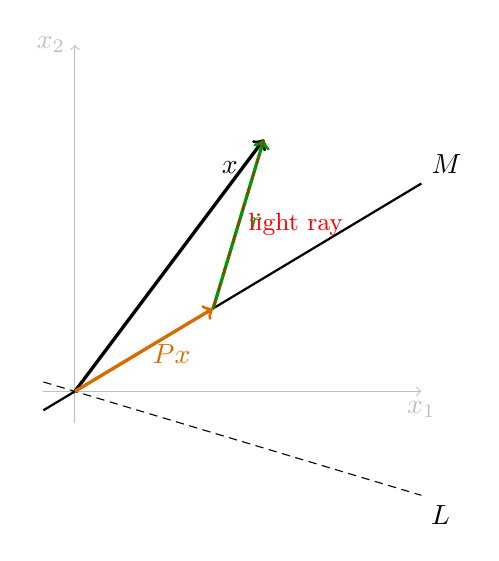
\begin{tikzpicture}[scale=2]
            % axes
            \draw[->,gray!50] (-0.2,0) -- (2.2,0) node[below] {$x_1$};
            \draw[->,gray!50] (0,-0.2) -- (0,2.2) node[left] {$x_2$};
            % Subspace M: y = 0.6 x
            \draw[thick] (-0.2,-0.12) -- (2.2,1.32) node[above right] {$M$};
            % Direction L: y = -0.3 x
            \draw[densely dashed] (-0.2,0.06) -- (2.2,-0.66) node[below right] {$L$};
            % Points/vectors
            \coordinate (O) at (0,0);
            \coordinate (X) at (1.2,1.6);
            \coordinate (PX) at (0.878,0.527); % oblique proj onto M along L
            % x and Px
            \draw[->,very thick] (O) -- (X) node[pos=0.82,above] {$x$};
            \draw[->,very thick,orange!85!black] (O) -- (PX) node[pos=0.7,below] {$Px$};
            % residual r (orthogonal to L)
            \draw[->,very thick,green!60!black] (PX) -- (X) node[midway,right] {$r$};
            % light ray along L
            \draw[dashed,red] (X) -- (PX) node[midway, right, red] {\small light ray};
        \end{tikzpicture}
        \caption*{\small Oblique: $r\perp L$ (not necessarily $\perp M$).}
    \end{minipage}
\end{figure}

\paragraph{Legend (mapping analogy \(\leftrightarrow\) math).}
\begin{itemize}
    \item Line \(M\): target subspace (“floor”). \quad Line \(L\): light direction (test space constraints).
    \item Arrow \(x\): original vector (“object”). \quad Arrow \(Px\): projection (“shadow”).
    \item Arrow \(r=x-Px\): drop vector from \(x\) to its shadow.
    \item Red dashed segment: “light ray” (perpendicular for orthogonal, tilted along \(L\) for oblique).
\end{itemize}



\section{Projections onto Subspaces}

The most important applications of projections involve projecting onto subspaces defined by sets of vectors or linear constraints.

\subsection{Projection onto Column Spaces}

Given a matrix $A  \in  \mathbb{R}^{m \times n}$ with linearly independent columns, we want to find the orthogonal projection onto $\text{Col}(A)$.

\begin{theorem}{Projection onto Column Space}{column-projection}
    Let $A  \in  \mathbb{R}^{m \times n}$ have linearly independent columns. Then the orthogonal projection onto $\text{Col}(A)$ is given by:
    \[
        P_A = A(A^{\top} A)^{-1} A^{\top}
    \]
    For any $\mathbf{b}  \in  \mathbb{R}^m$, the vector $P_A \mathbf{b}$ is the closest point in $\text{Col}(A)$ to $\mathbf{b}$ in the Euclidean norm.
\end{theorem}

\begin{proof}
    Let $P = A(A^{\top} A)^{-1} A^{\top}$. We verify the projection properties:

    \textbf{Idempotent:}
    \begin{align}
        P^2 & = A(A^{\top} A)^{-1} A^{\top} A(A^{\top} A)^{-1} A^{\top}   \\
            & = A(A^{\top} A)^{-1} (A^{\top} A)(A^{\top} A)^{-1} A^{\top} \\
            & = A(A^{\top} A)^{-1} A^{\top} = P
    \end{align}

    \textbf{Symmetric:}
    \[
        P^{\top} = (A(A^{\top} A)^{-1} A^{\top})^{\top} = A((A^{\top} A)^{-1})^{\top} A^{\top} = A(A^{\top} A)^{-1} A^{\top} = P
    \]

    \textbf{Range:} For any $\mathbf{x}  \in  \mathbb{R}^n$, $A\mathbf{x}  \in  \text{Col}(A)$ and $P(A\mathbf{x}) = A(A^{\top} A)^{-1} A^{\top} A\mathbf{x} = A\mathbf{x}$, so $\text{Col}(A) \subseteq \text{Range}(P)$. Since $P$ maps into $\text{Col}(A)$, we have equality.
\end{proof}

\begin{figure}[htb]
    \centering
     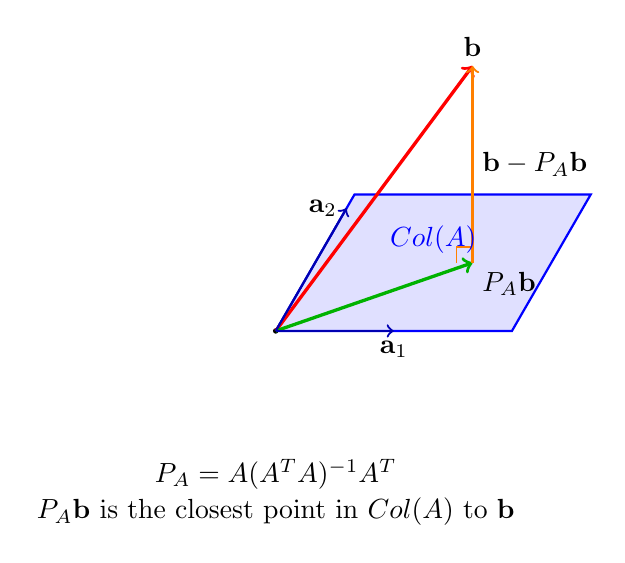
\begin{tikzpicture}[scale=1.0]
    % Set up 3D coordinate system
    \begin{scope}[x={(1cm,0cm)}, y={(0.5cm,0.866cm)}, z={(0cm,1cm)}]

        % Draw the column space as a plane
        \fill[blue!20, opacity=0.6] (0,0,0) -- (3,0,0) -- (3,2,0) -- (0,2,0) -- cycle;
        \draw[blue, thick] (0,0,0) -- (3,0,0) -- (3,2,0) -- (0,2,0) -- cycle;

        % Origin
        \fill[black] (0,0,0) circle (1pt);

        % Original vector b (outside the plane)
        \draw[red, very thick, ->] (0,0,0) -- (2,1,2.5);
        \node[above] at (2,1,2.5) {$\mathbf{b}$};

        % Projection P_A b onto the column space
        \draw[green!70!black, very thick, ->] (0,0,0) -- (2,1,0);
        \node[below right] at (2,1,0) {$P_A \mathbf{b}$};

        % Residual vector (b - P_A b)
        \draw[orange, thick, ->] (2,1,0) -- (2,1,2.5);
        \node[right] at (2,1,1.25) {$\mathbf{b} - P_A \mathbf{b}$};

        % Perpendicular indicator
        \draw[orange, thin] (1.8,1,0) -- (1.8,1,0.2) -- (2,1,0.2);

        % Column vectors of A
        \draw[blue!70!black, thick, ->] (0,0,0) -- (1.5,0,0);
        \node[below] at (1.5,0,0) {$\mathbf{a}_1$};
        \draw[blue!70!black, thick, ->] (0,0,0) -- (0,1.8,0);
        \node[left] at (0,1.8,0) {$\mathbf{a}_2$};

        % Label for the column space
        \node[blue] at (1.5,1,0.3) {$\text{Col}(A)$};

    \end{scope}

    % Equations
    \node[below] at (0,-1.5) {$P_A = A(A^T A)^{-1} A^T$};
    \node[below] at (0,-2) {$P_A \mathbf{b}$ is the closest point in $\text{Col}(A)$ to $\mathbf{b}$};
\end{tikzpicture}

    \caption{Projection onto the column space of a matrix $A$. The vector $\mathbf{b}$ is projected to $P_A \mathbf{b}$, the closest point in $\text{Col}(A)$.}
    \label{fig:column-projection}
\end{figure}

\subsection{Normal Equations}

The projection formula leads directly to the normal equations, fundamental to least squares problems.
\begin{equation}
    A^{\top} A \hat{\mathbf{x}} = A^{\top} \mathbf{b}
\end{equation}
Assume we have an overdetermined system $A\mathbf{x} = \mathbf{b}$ where $A  \in  \mathbb{R}^{m \times n}$ with $m > n$. The least squares solution minimizes $\|\mathbf{b} - A\mathbf{x}\|_2$.

\begin{corollary}{Normal Equations}{normal-equations}
    The projection of $\mathbf{b}$ onto $\text{Col}(A)$ is $A\hat{\mathbf{x}}$ where $\hat{\mathbf{x}}$ solves the normal equations:
    \[
        A^{\top} A \hat{\mathbf{x}} = A^{\top} \mathbf{b}
    \]
    This gives the least squares solution to the overdetermined system $A\mathbf{x} = \mathbf{b}$.
\end{corollary}

The geometric insight is that the residual $\mathbf{b} - A\hat{\mathbf{x}}$ must be orthogonal to $\text{Col}(A)$, leading to $A^{\top}(\mathbf{b} - A\hat{\mathbf{x}}) = 0$.


\subsection{QR Approach to Projections}

Using the QR decomposition $A = QR$ provides a numerically stable way to compute projections.

\begin{theorem}{QR-based Projection}{qr-projection}
    If $A = QR$ where $Q  \in  \mathbb{R}^{m \times n}$ has orthonormal columns and $R  \in  \mathbb{R}^{n \times n}$ is upper triangular, then:
    \[
        P_A = QQ^{\top}
    \]
    The projection of $\mathbf{b}$ onto $\text{Col}(A)$ is simply $QQ^{\top} \mathbf{b}$.
\end{theorem}

This approach avoids forming $A^{\top} A$ and leverages the excellent numerical properties of orthogonal matrices.
